\documentclass{article}

\usepackage[T1]{fontenc}
\usepackage[polish]{babel}
\usepackage[utf8]{inputenc}
\usepackage{lmodern}
\usepackage{indentfirst}
\usepackage{listings}
\usepackage{enumitem}
\usepackage{pdfpages}
\usepackage{hyperref}
\selectlanguage{polish}

\title{Markov Monster Chat \\
Specyfikacja implementacyjna}
\author{Adrian Zdanowicz}

\begin{document}

\maketitle


UWAGA: Poniższy dokument utworzony został w oparciu o wczesną koncepcję programu.
Niektóre z zawartych w nim założeń oraz opisywane sposoby użycia mogą
ulec zmianie w późniejszej fazie tworzenia projektu.


\section{Język}

Program \textbf{Markov Monster Char} napisany jest w języku Java przy użyciu środowiska IntelliJ IDEA.


\section{Zewnętrzne biblioteki}

Powłoka graficzna programu tworzona jest z pomocą biblioteki Swing.

\section{Struktury danych}

Program podzielony będzie na dwa główne pakiety - \textbf{monster} oraz \textbf{gui}.

\subsection{monster}

Pakiet \textbf{monster} spaja klasy, które implementują rdzeń programu - funkcjonalność
analogiczną do tej oferowanej przez projekt stworzony w języku C.

Głównym elementem pakietu jest klasa \textbf{Monster}, która funkcjonuje jako główna klasa pakietu. Tak jak w projekcie w jęz. C, przechowuje ona ustawienia generatora oraz zawiera klasy \textbf{Pool} (przechowującą dane o słowach) oraz \textbf{MarkovGen} (przechowującą dane o n-gramach).

Publiczne metody udostępniane przez \textbf{Monster}:

\begin{lstlisting}[frame=single]
void ReadTextFiles(String[] fileNames);
void GenerateStats();
void ReadDictionaryFiles(String[] fileNames);
void GenerateDictionaryFile(String fileName);

// Do czytania oraz generowania odpowiedzi
void ReadChatLine(String line);
String GenerateNextChatLine();
\end{lstlisting}

Dla uproszczenia programu, pole przechowujące referencję na klasę Pool będzie dostępne
dla innych klas, dzięki temu w razie potrzeby pakiet \textbf{gui} może odczytać statystyki bezpośrednio z publicznych pól klasy Pool bez potrzeby wprowadzania nowych typów danych.

Klasa \textbf{Pool} została uproszczona względem implementacji w języku C
(ponieważ Java udostępnia struktury danych, które poprzednio implementowano w Pool
ręcznie) i teraz jest głównie wrapperem wokół wektora klas WMEntry:

\begin{lstlisting}[frame=single]
public class WWEntry
{
	public String		rawWord;
	public int			wordHash;
	public int			index;
	
	public void			weHaveUsedAWord();
};
\end{lstlisting}

\subsection{gui}

Pakiet \textbf{gui} składa się z klas wygenerowanych przez środowisko podczas generowania okienka programu. Action listenery wykonują operacje, wywołując odpowiednie metody z pakietu \textbf{monster}.


\section{Diagram klas}

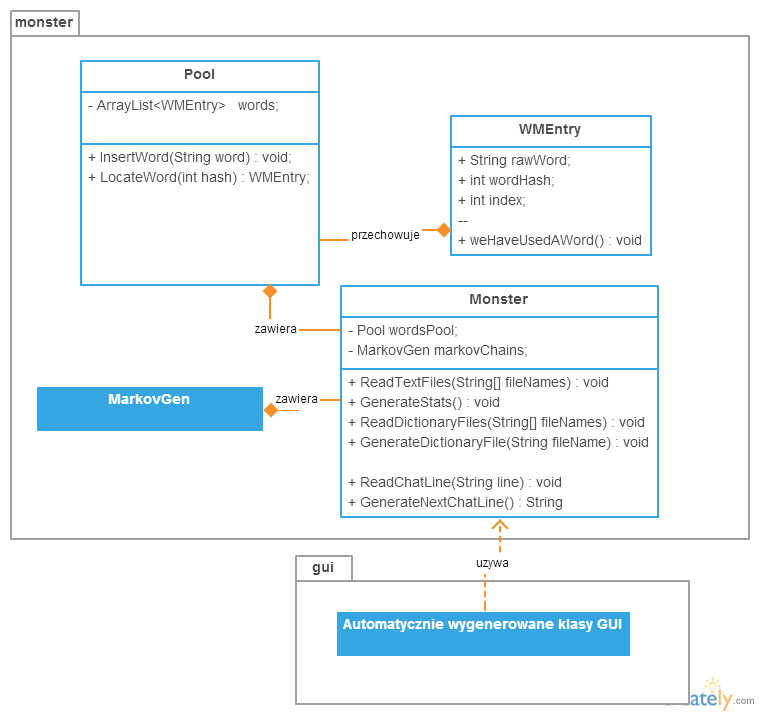
\includegraphics[width=\textwidth]{MMChat_diag.png}


\section{Wzorce projektowe}

Kluczową rolę przy tworzeniu kodu programu odgrywa fasada, ukrywająca implementację klas.
Fasada zostanie zastosowana na kilku poziomach, tj. ukryta zostanie zarówno implementacja
głównej klasy Monster, jak i (w miarę możliwości) klas używanych przez nią.

Z racji braku potrzeby polimorfizmu, w projekcie nie znajdą zastosowania bardziej
złożone wzorce projektowe, takie jak np. fabryka.


\section{Interfejs programu}

Interfejs programu w całości realizowany jest przez powłokę graficzną, prezentowaną
wcześniej w specyfikacji funkcjonalnej.


\section{Testy}

By zweryfikować poprawność wytworzonego kodu, do klas stworzone zostaną testy jednostkowe.
Przewidziane jest głównie bezpośrednie testowanie klasy Monster, jednak w przypadku
wystąpienia jakichkolwiek problemów z klasami, na których zależy główny moduł, zostaną
dopisane do nich odpowiednie testy. Mowa tu głównie o testach poprawności operowania na
kontenerze słów oraz poprawności generowania łańcuchów Markova.

Interfejs graficzny będzie testowany ręcznie.

\end{document}